\chapter{宽带调制信号的自动识别}\label{chap:intro}
\markboth{第四章\ \ 宽带调制信号的自动识别}{}
% 宽带亚采样信号的自动识别
% 第四章“宽带亚采样调制信号的自动识别”可以按照以下大纲进行组织:

% 1. **引言**
%    - 介绍研究背景和宽带亚采样调制信号自动识别的重要性。
%    - 阐述研究动机和本章的目的。

% 2. **理论基础和相关工作**
%    - 介绍亚奈奎斯特采样和自动调制识别的基本概念。
%    - 回顾相关领域的研究进展和现有技术。

% 3. **单用户通信场景下的调制识别**
%    - 描述单用户场景的问题设定和挑战。
%    - 介绍使用AD-AMR Net模型进行调制识别的方法和策略。

% 4. **多用户通信场景下的调制识别**
%    - 讨论多用户场景的特点和复杂性。
%    - 介绍三种不同的调制识别方案:直接预测、分步骤方法和多任务学习。

% 5. **实验设计和结果分析**
%    - 描述实验设置、所用数据集和评估指标。
%    - 展示实验结果,并进行详细分析。

% 6. **讨论**
%    - 分析各种方法的优缺点和适用性。
%    - 探讨研究结果对于实际应用和理论发展的意义。

% 7. **结论和未来工作**
%    - 总结本章的主要发现和贡献。
%    - 提出未来研究的方向和可能的改进。

% 这个大纲旨在全面覆盖宽带亚采样调制信号自动识别的关键方面,从理论基础到实际应用,以及从单用户到多用户场景的不同识别策略,为读者提供一个清晰、连贯的研究框架。

% 宽带信号的调制识别可以分为两个方向,一种是只有一个用户在通信的场景,这个时候只需要识别其调制模式即可,另一种是有多个用户在通信的场景,这个时候需要同时识别其所在的子带位置和所使用的调制模式,由第三章的实验,我们提出了一种AD-AMR Net用于调制识别,在这一章节中我们可以将其用作backbone,针对单用户场景只需要对问题进行建模,选择合适的预处理方式,然后在分析性能即可,而多用户场景则比较困难,目前鲜有相关的研究,所以我们需要讨论多种方案,在本章中我们针对该问题采用了三个不同的方案,第一个方案是根据子带的情况和各种调制的可能性,直接预测相应的所有情况,这种方案比较容易实现,可以作为一个基线,第二种方案则是分多步来进行,先识别子带的位置,然后在得到位置信息后进一步进行调制的识别,第三种则是多任务的形式,先总体地对亚采样信号进行特征提取,然后再用不同的head分别实现子带位置的判别和调整模式的识别,与前者不同的是,第三种方案共用了一个特征提取模块,减少了模型的复杂度,同时增加了两个子任务的关联性

\section{引言}\label{sec:background}

在现代通信系统中,频谱资源的有效利用成为了一个关键挑战。随着物联网和无线通信技术的迅速发展,对于高效的频谱利用和信号处理方法的需求日益增长。在这种背景下,亚奈奎斯特采样作为一种有效的频谱感知技术,能够在较低的采样率下捕获宽带信号,减少处理高速信号所需的资源和成本。

自动调制识别在提高通信系统的灵活性和效率方面发挥着重要作用。特别是在多用户通信和动态频谱访问环境中,能够快速准确地识别不同用户的调制方式是至关重要的。然而,当涉及到宽带亚采样信号时,传统的调制识别方法面临着新的挑战,例如如何在降低的采样率下维持识别精度。

在本章节中,我们聚焦于宽带信号的调制识别,这一任务可以分为两个主要方向。首先是单用户通信场景,其中核心任务是识别特定用户的调制模式。针对这一场景,我们利用第三章中提出的AD-AMR Net和主流深度学习模型作为主干网络,通过对问题进行合理的建模和选择适当的预处理方法,进而分析模型在单用户调制识别任务上的性能。

另一方面,我们探讨了更为复杂的多用户通信场景,这一场景不仅要求识别调制模式,还需要确定通信信号的子带位置。由于这一领域的研究相对较少,我们在本章中采用了三种不同的方案来应对这一挑战。第一个方案是直接预测各种可能的子带位置和调制模式的组合,这种方法较为直接,可作为基线模型。第二种方案采用分步骤方法,即先识别子带位置,再基于位置信息进行调制模式的识别。第三种方案则采用多任务学习的形式,通过共享的特征提取模块来同时实现子带位置判别和调制模式识别,这种设计既减少了模型复杂度,也增强了两个子任务之间的关联性。

通过这一章节的研究,我们旨在提供有效的解决方案来应对宽带亚采样调制信号识别中的挑战,同时推动无线通信技术在频谱效率和智能信号处理方面的进步。这不仅对于解决现实世界的通信问题至关重要,也对于理论研究和技术创新具有重要的指导意义。

\begin{figure}
    \centering
    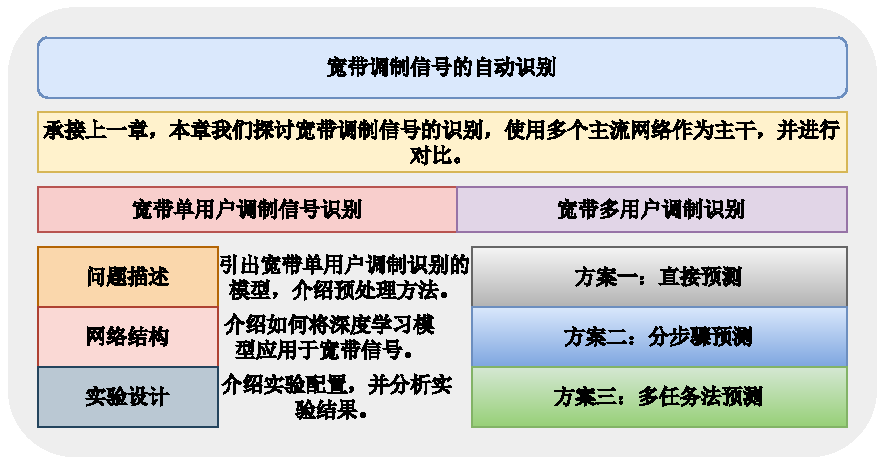
\includegraphics[width=\textwidth]{Image/chap4_map.pdf}
    \caption{本章脉络}
    \label{fig:chap4_overview}
\end{figure}

\section{宽带单用户调制信号识别}\label{sec:background}
% 在撰写单用户场景下的调制识别部分时,您可以按照以下思路来组织内容:

% 1. **问题描述和挑战**:
%    - 介绍单用户通信场景的特点。
%    - 描述在亚奈奎斯特采样条件下进行调制识别所面临的技术挑战。

% 2. **方法论**:
%    - 阐述使用AD-AMR Net进行调制识别的整体方法论。
%    - 详细描述数据预处理、特征提取和分类器设计的步骤。

% 3. **模型架构**:
%    - 详细介绍模型的架构,包括各层的功能和配置。
%    - 插图:提供模型架构的示意图,展示不同层级和组件的关系。

% 4. **实验设置**:
%    - 描述实验的具体设置,包括数据集的选择、模型的训练和评估指标。
%    - 插图:可展示部分样本数据的波形图或频谱图,以帮助理解数据特性。

% 5. **结果分析**:
%    - 展示模型在单用户场景下的识别结果。
%    - 分析模型性能,讨论其在不同条件下的表现。

% 6. **比较与讨论**:
%    - 将AD-AMR Net的性能与其他方法进行比较。
%    - 讨论模型在单用户场景下的优势和局限性。

% 7. **结论**:
%    - 总结在单用户场景下调制识别的主要发现。
%    - 提出可能的改进方向和后续工作的建议。

% 通过这样的结构,您可以系统地介绍单用户场景下调制识别的方法、实验过程和结果分析,为读者提供深入的理解,并展示您的研究成果。

\subsection{问题描述和挑战}\label{sec:background}

\begin{figure}
    \centering
    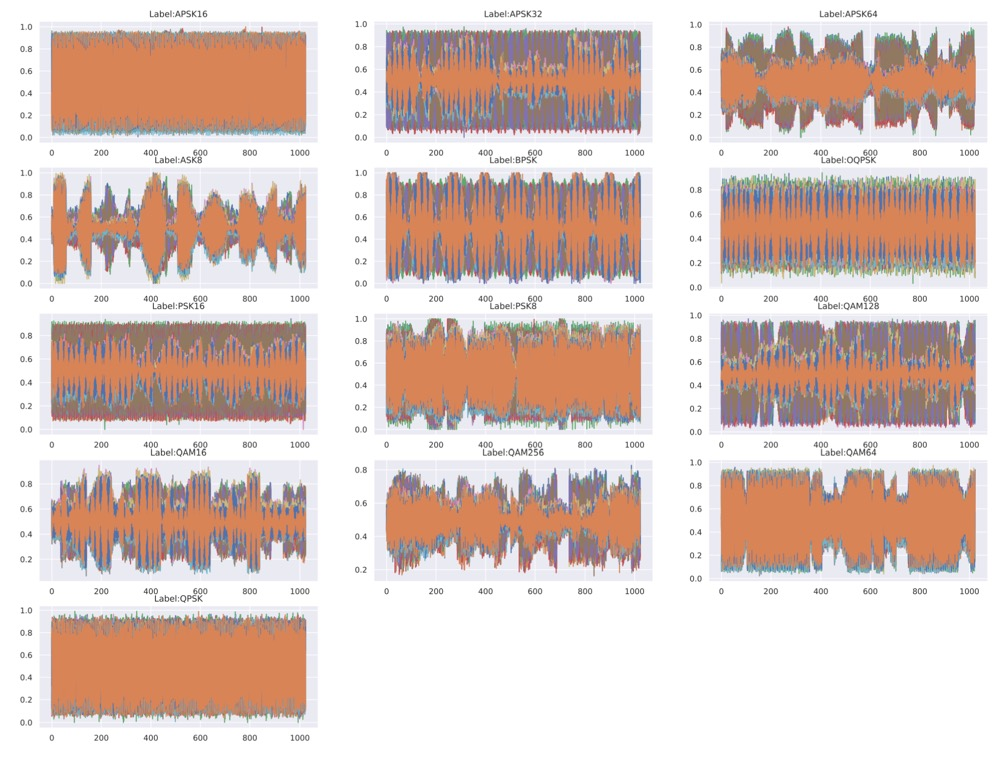
\includegraphics[width=0.8\textwidth]{Image/modulations.jpg}
    \caption{宽带欠采样信号的可视化}
    \label{fig:modulations}
\end{figure}

在宽带单用户调制信号识别的实验研究中,我们集中关注于数据预处理方法、问题建模策略以及AD-AMR Net模型的应用。考虑到亚奈奎斯特采样信号的特点,我们采纳了\textbf{Min-max}预处理方法,\textbf{Min-max}的数学表达式如下:

\begin{equation}
    \boldsymbol{x}_\text{\emph{norm}} = \frac{\boldsymbol{x} - \min(\boldsymbol{x})}{\max(\boldsymbol{x}) - \min(\boldsymbol{x})},
\end{equation}
其中$\boldsymbol{x}_{min}$和$\boldsymbol{x}_{max}$分别表示信号的最小值和最大值。这种方法可以将信号的幅度归一化到$[0, 1]$的范围内,从而保证数据的稳定性和可靠性。以确保在保持数据基本特性的同时,使之适合于神经网络的处理需求。具有不同延迟特性的八个模数转换器(ADC)负责收集输入数据,这些ADC的延迟值为16, 11, 1, 0, 27, 24, 37, 31。这种独特的延迟配置为信号采集引入了额外的复杂性。数据以$I_1, Q_1, I_2, Q_2, ..., Q_8$的顺序排列,构成一个$16 \times 1024$的矩阵,其中I和Q分别表示信号的同相分量和正交分量。此外,我们的研究涵盖了13种调制类型,包括APSK16, APSK32, APSK64, ASK8, BPSK, OQPSK, PSK16, PSK8, QAM128, QAM16, QAM256, QAM64, QPSK等,增加了识别任务的复杂度。宽带欠采样信号的可视化如图\ref{fig:modulations}所示。

在这些背景下,我们面临的主要挑战是有效处理由不同延迟的ADC采集的复杂信号,并从中准确识别出多种可能的调制类型。这不仅要求精确的数据预处理,还需要强大的分类算法,以在降低采样率的条件下实现高精度的调制识别。本章实验设计的目标是分析不同的深度学习模型在处理单用户场景下宽带亚采样信号时的有效性,以及评估其在特定条件下的表现。通过这些实验,我们将深入探索模型在实际应用中的潜力和局限性,为宽带信号的调制识别领域提供新的见解。、

本节中,我们专注于单用户场景下的宽带信号特征提取能力的比较研究。考虑到单用户场景相对简单,它为评估不同深度学习模型在宽带信号处理上的性能提供了一个理想的测试环境。为此,我们选取了多种主流的深度学习模型进行比较,包括传统的ResNet、加入了卷积层注意力模块(Convolutional Block Attention Module, CBAM)的ResNet、融合了自注意力机制的卷积神经网络、加入了残差收缩模块(Residual Shrinkage Block)的ResNet,以及第三章中提出的集成了高效通道注意力的残差收缩模块的ResNet。通过这一系列的比较分析,我们可以深入理解每个模型在宽带信号特征提取方面的优势和局限,为自动调制识别技术的发展提供新的见解。

\subsection{网络结构}\label{sec:background}


\begin{figure}
    \centering
    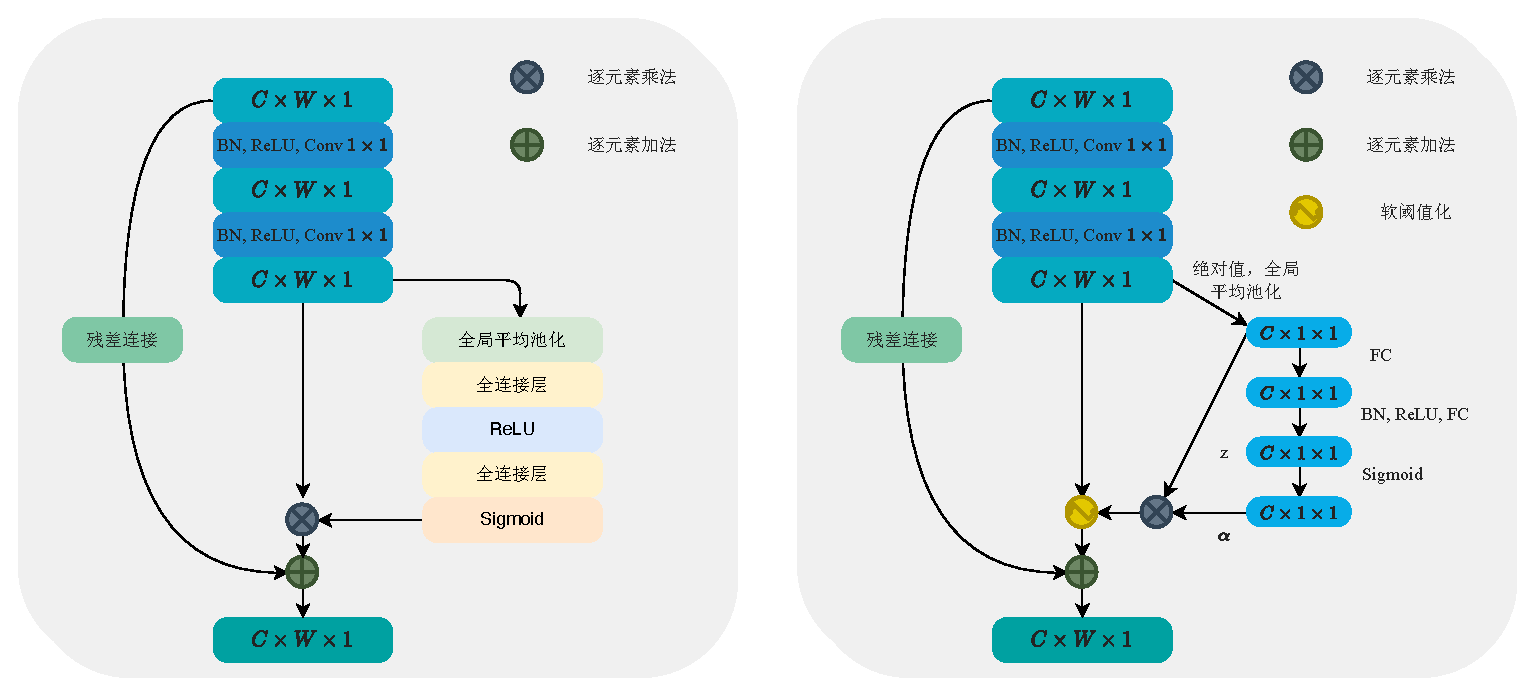
\includegraphics[width=\textwidth]{Image/se_rsb_cn.pdf}
    \caption{挤压-激励模块(左)和残差收缩模块(右)}
    \label{fig:se_rsb}
\end{figure}

\subsubsection{挤压-激励模块}\label{sec:background}
在深度学习领域,特别是在图像识别和信号处理任务中,注意力机制的引入已经证明可以显著提升模型的性能。挤压-激励模块(Squeeze-and-Excitation, SE)是一种有效的注意力机制实现,它通过重新校准卷积层的特征通道的响应强度,增强了模型对于重要特征的关注度,同时抑制了不重要的特征。SE模块的核心思想是先对特征图进行全局平均池化(Squeeze),从而生成特征通道的全局描述,然后通过两个全连接层(Excitation)对这些描述进行重标定,最终通过缩放原始特征图来实现特征的重新校准。这个过程可以表示为:

\begin{equation}
    \textbf{S}(z) = \frac{1}{H \times W} \sum_{i=1}^{H} \sum_{j=1}^{W} z_{i,j}
\end{equation}
\begin{equation}
    \textbf{E}(s) = \sigma(g(s, \textbf{W})) = \sigma(\textbf{W}_2 \delta(\textbf{W}_1 s))
\end{equation}
\begin{equation}
    \tilde{x}_c = F_{scale}(x_c, e_c) = e_c \cdot x_c
\end{equation}

其中,\(z\) 是输入特征图,\(\textbf{S}(z)\) 表示Squeeze操作后的全局特征,\(\textbf{E}(s)\) 是Excitation操作后的权重系数,\(\sigma\) 表示sigmoid激活函数,\(g\) 表示全连接层操作,\(\textbf{W}_1\) 和 \(\textbf{W}_2\) 是全连接层的权重,\(\delta\) 表示ReLU激活函数,\(e_c\) 是每个通道的重标定权重,\(\tilde{x}_c\) 是最终的输出特征图,\(F_{scale}\) 表示特征缩放函数。

为了将SE模块应用于一维信号处理任务中,特别是调制识别,我们对其进行了适当的修改,将原本针对二维图像特征的处理改为适用于一维信号。这意味着在Squeeze阶段,我们采用一维全局平均池化而不是二维平均池化,以正确地处理一维信号数据。这种改进使得SE模块能够有效地处理一维信号特征,通过学习到的通道权重来强调重要的信号特征并抑制不相关的噪声或信息,从而提高了调制识别任务的性能。

将SE模块运用于该任务上,我们的理念是利用其通道注意力机制来增强神经网络对一维信号中重要特征的捕捉能力,进一步提升调制识别的准确性。通过对一维信号特征的有效校准,我们能够实现对信号中调制特征的更加精确识别,这对于提高无线通信系统中的信号处理性能至关重要。

\subsubsection{残差收缩模块}\label{sec:background}
在深度探索深度学习模型在信号处理领域,特别是调制识别任务的应用中,残差收缩模块(Residual Shrinkage Block, RSB)凭借其独特的优势成为研究的焦点。该模块,如图\ref{fig:se_rsb}所示,通过整合残差连接和特征收缩机制,显著优化了网络的特征学习流程并增强了特征表达能力,使得RSB在复杂信号处理任务中展现出非凡的性能。

RSB模块的一大创新在于其对软阈值化技术的应用,这是信号处理中一种常用的工具,特别适合于处理含有噪声的信号。软阈值化通过设置一个阈值来减少信号中的小波系数,有效地去除噪声同时保留信号的主要特征。这一过程中,阈值的选择至关重要——过高会导致信号的过度平滑,损失有价值信息;而过低则可能无法充分去除噪声。RSB通过融入神经网络,能够自适应地学习和调整软阈值化中的阈值参数,从而在去噪和特征保留之间实现最佳平衡。

这种自适应的软阈值化机制,使得RSB在处理宽带信号调制识别任务时尤其有效。宽带信号常包含复杂的调制特征和背景噪声,RSB能够有效地从这些信号中提取出关键信息,抑制不必要的干扰,进而提高调制识别的准确度和鲁棒性。动态调整特征通道,加之其强化关键特征的学习能力,使RSB在复杂信号处理中显示出优越的性能。

正是基于RSB在特征提取、信息压缩及网络训练稳定性方面的显著优势,以及其在软阈值化应用中的自适应能力,我们选择将其作为对比研究对象之一。此项比较旨在全面评估RSB模块在宽带信号处理,尤其是调制识别任务中的表现。通过这种方式,我们不仅能够验证RSB模块的实际效用,也为深度学习模型处理高复杂度信号的未来研究提供新的视角和方法。

\subsubsection{卷积层注意力模块(CBAM)}\label{sec:background}

\begin{figure}
    \centering
    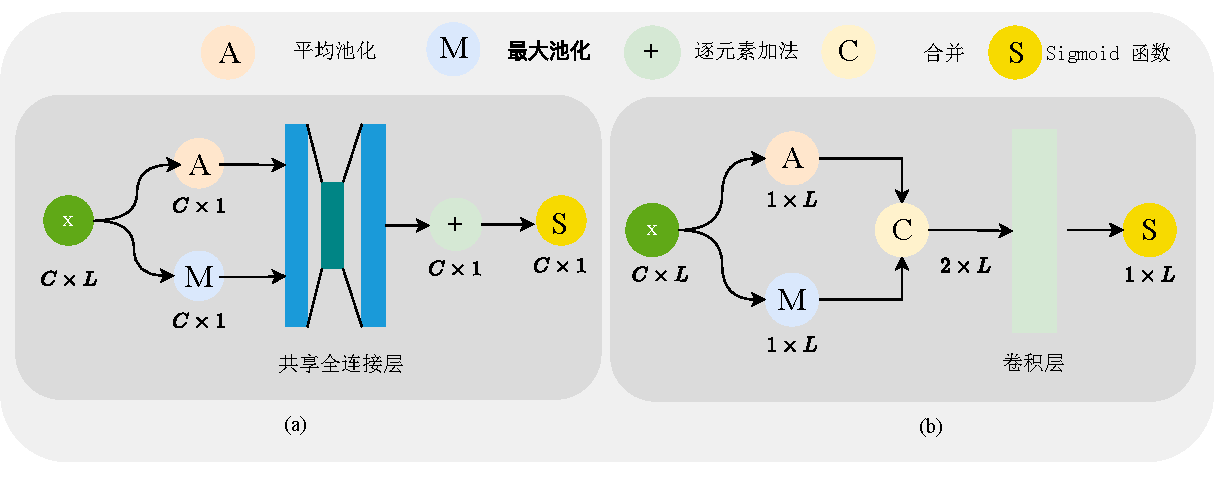
\includegraphics[width=\textwidth]{Image/CBAM_cn.pdf}
    \caption{卷积块注意力模块(CBAM)}
    \label{fig:cbam}
\end{figure}

CBAM(Convolutional Block Attention Module)图\ref{fig:cbam}是一种用于增强神经网络特征表达能力的注意力机制模块。它通过对输入特征图进行细致的分析,有效地强调了对任务有益的特征,从而提升了网络的整体性能。CBAM的核心设计理念是在通道和空间两个维度上应用注意力机制,以此优化网络的特征学习过程\cite{woo2018cbam}。

通道注意力机制关注于识别并强调那些对最终识别任务最重要的通道。它通过全局平均池化和最大池化操作来捕获通道间的全局信息,然后通过多层感知机(MLP)和激活函数来生成通道注意力权重。这个过程可以理解为一种自动的特征选择机制,使网络更加专注于有助于任务的特征通道。通道注意力的计算公式如下:

\begin{equation}
    \begin{aligned}
    M_c(F) &= \sigma(MLP(AvgPool(F)) + MLP(MaxPool(F))) \\ 
    &= \sigma(W_1(W_0(F_{avg}^c)) + W_2(W_0(F_{\max}^c)),
    \end{aligned}
    \label{equ:CAM}
\end{equation}
其中$F$表示输入特征图,$F_{avg}^c$和$F_{\max}^c$分别表示$F$的通道$c$的平均池化和最大池化结果,$W_0$和$W_1$表示两个MLP的权重矩阵,$\sigma$表示激活函数,$M_c(F)$表示通道注意力权重。通过这种方式,网络可以自动学习到每个通道的重要性,从而提高特征的表达能力。

空间注意力机制则集中于特征图的特定空间区域。它通过池化操作来总结特征图的空间信息,并通过一个小型的卷积层来生成空间注意力图。这一机制有助于突出重要的空间区域,使网络能够更加关注于对分类或其他任务有利的空间特征。空间注意力的计算公式如下:

\begin{equation}
    \begin{aligned}
    M_s(F) &= \sigma(f^{7}([AvgPool(F), MaxPool(F)])) \\
    &= \sigma(f^{7}([F_{avg}^s, F_{\max}^s])
    \end{aligned}
    \label{equ:SAM}
\end{equation}
其中$F_{avg}^s$和$F_{\max}^s$分别表示$F$的平均池化和最大池化结果,$f^7$表示一个$7 \times 7$的卷积层,$M_s(F)$表示空间注意力权重。通过这种方式,网络可以自动学习到每个空间区域的重要性,从而提高特征的表达能力。

\begin{figure}
    \centering
    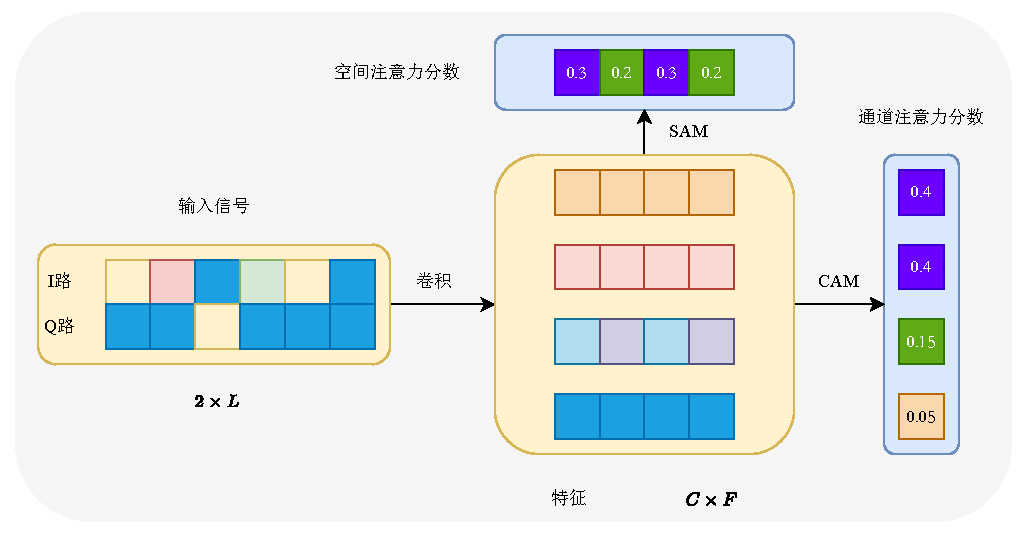
\includegraphics[width=\textwidth]{Image/cbam_on_iq.pdf}
    \caption{卷积块注意力模块用于IQ信号的特征提取}
    \label{fig:cbam_iq}
\end{figure}

原始的CBAM设计是针对二维特征图的,主要用于计算机视觉领域。为了适应一维的信号处理任务,例如调制识别,CBAM模块经过了适当的修改。在这种情况下,CBAM的设计需要考虑信号的时域特性,并根据一维数据的结构进行调整。例如,通道注意力机制可以专注于不同时间窗口内的信号特征,而空间注意力机制则可以针对信号的不同部分进行加权,这对于捕获时间序列数据的重要模式尤为关键。图\ref{fig:cbam_iq}展示了卷积模块注意力机制在处理IQ信号时的大概过程,旨在通过计算空间注意力分数和通道注意力分数来增强模型对信号的识别能力。图中首先展示了输入信号,分为I路和Q路,这两路信号代表了复信号的实部和虚部,是无线通信中常用的信号表示方法。
在经过初步的卷积操作后,模型分别对处理过的信号应用了空间注意力机制和通道注意力机制。空间注意力机制(SAM)通过聚焦于信号中最重要的空间区域来增强特征表达,其注意力分数如图中所示,是通过评估信号各部分的重要性后得到的权重分布,例如0.3、0.2等。这种机制能够使模型更加关注于信号中具有较高信息含量的区域。通道注意力机制(CAM)则关注于不同通道(在本例中可以理解为I路和Q路信号的不同特征通道)的重要性,通过为每个通道分配一个注意力分数(如图中的0.4、0.15、0.05)来实现。这允许模型对不同的特征通道进行重标定,从而强化重要通道的特征而抑制不重要通道的特征。整个过程最终导致了对输入IQ信号特征的有效提炼和加强,使得模型能够更加准确地识别和处理信号。

CBAM的优点在于其模块化和灵活性。它可以轻松地嵌入到现有的卷积神经网络中,无需对网络架构进行大规模修改。此外,CBAM对于不同类型的神经网络,如ResNet或CNN,都有良好的兼容性。在应用于一维信号处理任务时,CBAM提供了一种有效的方式来增强网络对时间序列数据的理解能力,从而提高整体性能。

\subsubsection{自注意力与多头自注意力机制}\label{sec:background}

\begin{figure}
    \centering
    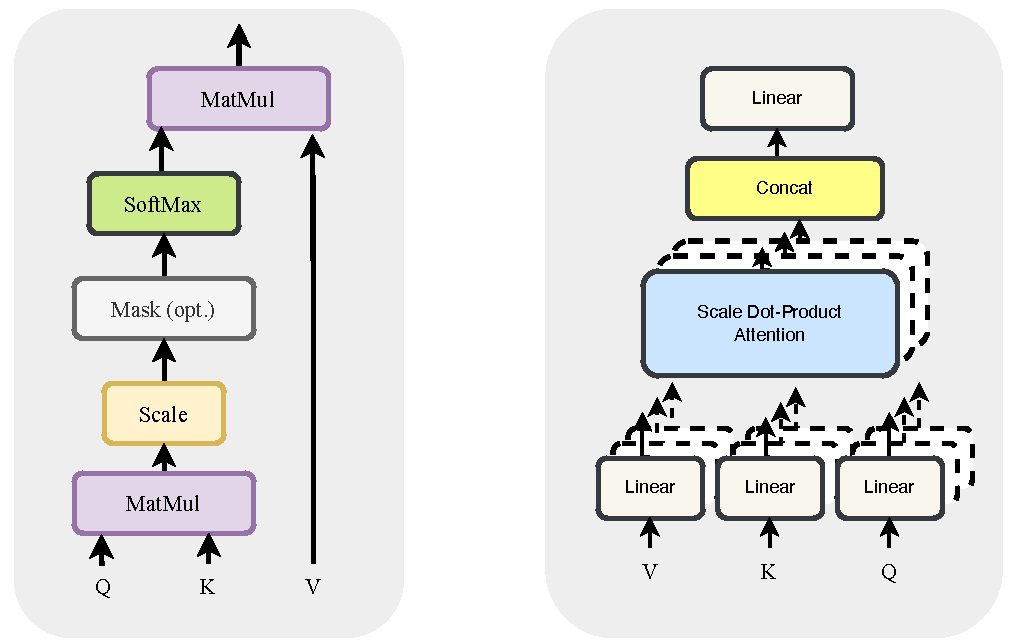
\includegraphics[width=\textwidth]{Image/self-attention.pdf}
    \caption{自注意力与多头自注意力机制}
    \label{fig:self-attention}
\end{figure}

自注意力机制和多头自注意力机制图\ref{fig:self-attention}是深度学习中用于增强模型处理序列数据能力的重要技术。这些机制在处理如自然语言和复杂信号等序列数据时尤为有效。

自注意力机制的核心在于允许模型在处理序列中的每个元素时,同时考虑序列中的所有其他元素。这种机制通过计算序列中每个元素与其他元素之间的关系强度来实现,从而使模型能够更好地理解和表示序列数据。具体来说,自注意力机制通过计算“查询”(Query)、“键”(Key)和“值”(Value)三个向量的相互作用来实现,这些向量是通过对输入数据的不同变换得到的。自注意力的计算过程涉及到这些向量间的点乘操作,然后通过softmax函数进行归一化,从而得到不同元素间的注意力权重。通过这种方式,模型可以更加关注与当前处理元素最相关的其他元素。其计算公式如下:

\begin{equation}
    \text{Attention}(Q, K, V) = \text{softmax}(\frac{QK^T}{\sqrt{d_k}})V,
\end{equation}
其中$d_k$表示“键”向量的维度。

多头自注意力机制则是在此基础上的拓展。它包含多个自注意力“头”,每个头都执行自注意力操作,但使用不同的参数。这样,模型可以从不同的表示子空间中学习信息,从而获得更加全面和丰富的数据表示。每个头的输出会被合并并通过一个线性层进行转换,以产生最终的输出。这种设计使得模型可以在多个维度上捕获序列数据的特征,从而增强了模型的表达能力。其计算公式如下:

\begin{equation}
    \text{MultiHead}(Q, K, V) = \text{Concat}(\text{head}_1, ..., \text{head}_h)W^O,
\end{equation}
其中$\text{head}_i = \text{Attention}(QW_i^Q, KW_i^K, VW_i^V)$,$W_i^Q, W_i^K, W_i^V$和$W^O$分别表示第$i$个头的“查询”、“键”、“值”和输出的线性变换矩阵。

在宽带信号调制识别的应用中,这些机制尤为重要。自注意力和多头自注意力机制可以帮助模型更有效地处理和分析宽带信号中的复杂模式和结构,如频率变化、时间依赖性等。通过这些机制,模型能够更准确地识别不同的调制类型和信号特性,即使在信噪比较低或者信号受到干扰的情况下也是如此。因此,我们将这些机制应用于宽带信号调制识别的任务中,以研究它们对于提高模型性能的作用。


\begin{figure}
    \centering
    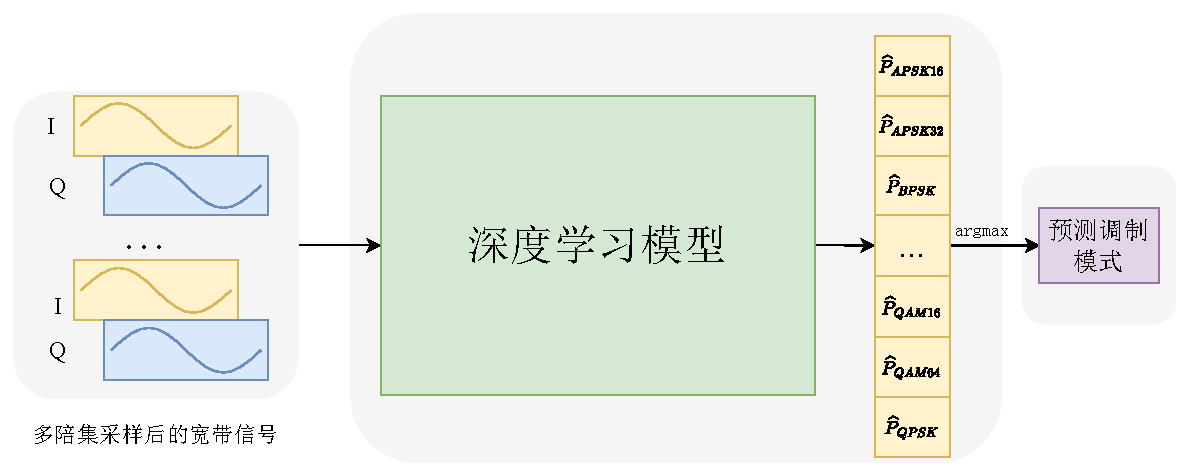
\includegraphics[width=\textwidth]{Image/adamr-wideband.pdf}
    \caption{单用户通信场景下的调制识别网络结构}
    \label{fig:basic}
\end{figure}

\subsection{实验设置}\label{sec:background}

本实验的目的是评估和比较不同模型在调制识别任务上的性能。我们选择了基于PyTorch框架在Ubuntu系统上进行的实验,并使用了NVIDIA RTX 3090 GPU来加速模型训练过程。实验数据集采用的是专为调制识别设计的GBSense 2022 Basic,它包含了多种调制类型的信号样本。

为了确保实验的公平性,我们设定了以下实验条件:

\begin{itemize}
    \item \textbf{对比模型}:我们以ResNet作为基线模型,并评估了几种主流的注意力机制模块——SE模块、RSB模块、CBAM模块、多头自注意力机制模块,以及我们自行提出的AD-AMR Net。这样做是为了观察这些模型在调制识别任务上的性能表现。
    \item \textbf{实验平台}:实验在Ubuntu操作系统上,基于PyTorch框架执行。我们利用NVIDIA RTX 3090 GPU加速了训练过程,以提高实验效率。
    \item \textbf{数据集}:使用GBSense 2022 Basic数据集进行训练、验证和测试,数据集被划分为训练集(60\%)、验证集(20\%)和测试集(20\%)。
    \item \textbf{训练细节}:所有模型都将被训练100个epochs,以确保足够的学习。我们引入了早停机制(Early Stopping)以防过拟合,以及平台期衰减学习率(ReduceLROnPlateau)机制,以自适应调整学习率,确保有效的学习率调整。
    \item \textbf{优化器与损失函数}:在训练过程中,我们采用了随机梯度下降(SGD)优化器,并使用交叉熵损失函数(Cross-Entropy Loss)作为模型训练的损失函数,这有助于处理分类问题中的多类标签。
\end{itemize}

\subsection{评价指标}

模型的性能将基于以下关键指标进行评估:

\begin{itemize}
    \item \textbf{模型参数量}:反映模型复杂度的指标,较少的参数量意味着模型更为简洁。
    \item \textbf{训练至收敛的Epoch数}:衡量模型训练效率的指标,较少的Epoch数表示模型训练所需时间更短。
    \item \textbf{最终准确率}:衡量模型性能的主要指标,在测试集上的准确率越高,表示模型性能越好。
\end{itemize}

通过这些评价指标,我们不仅能够客观比较各模型的性能,还能深入分析各种注意力机制在调制识别任务中的实际应用效果和价值。


\subsection{结果分析}\label{sec:background}

\begin{figure}
    \centering
    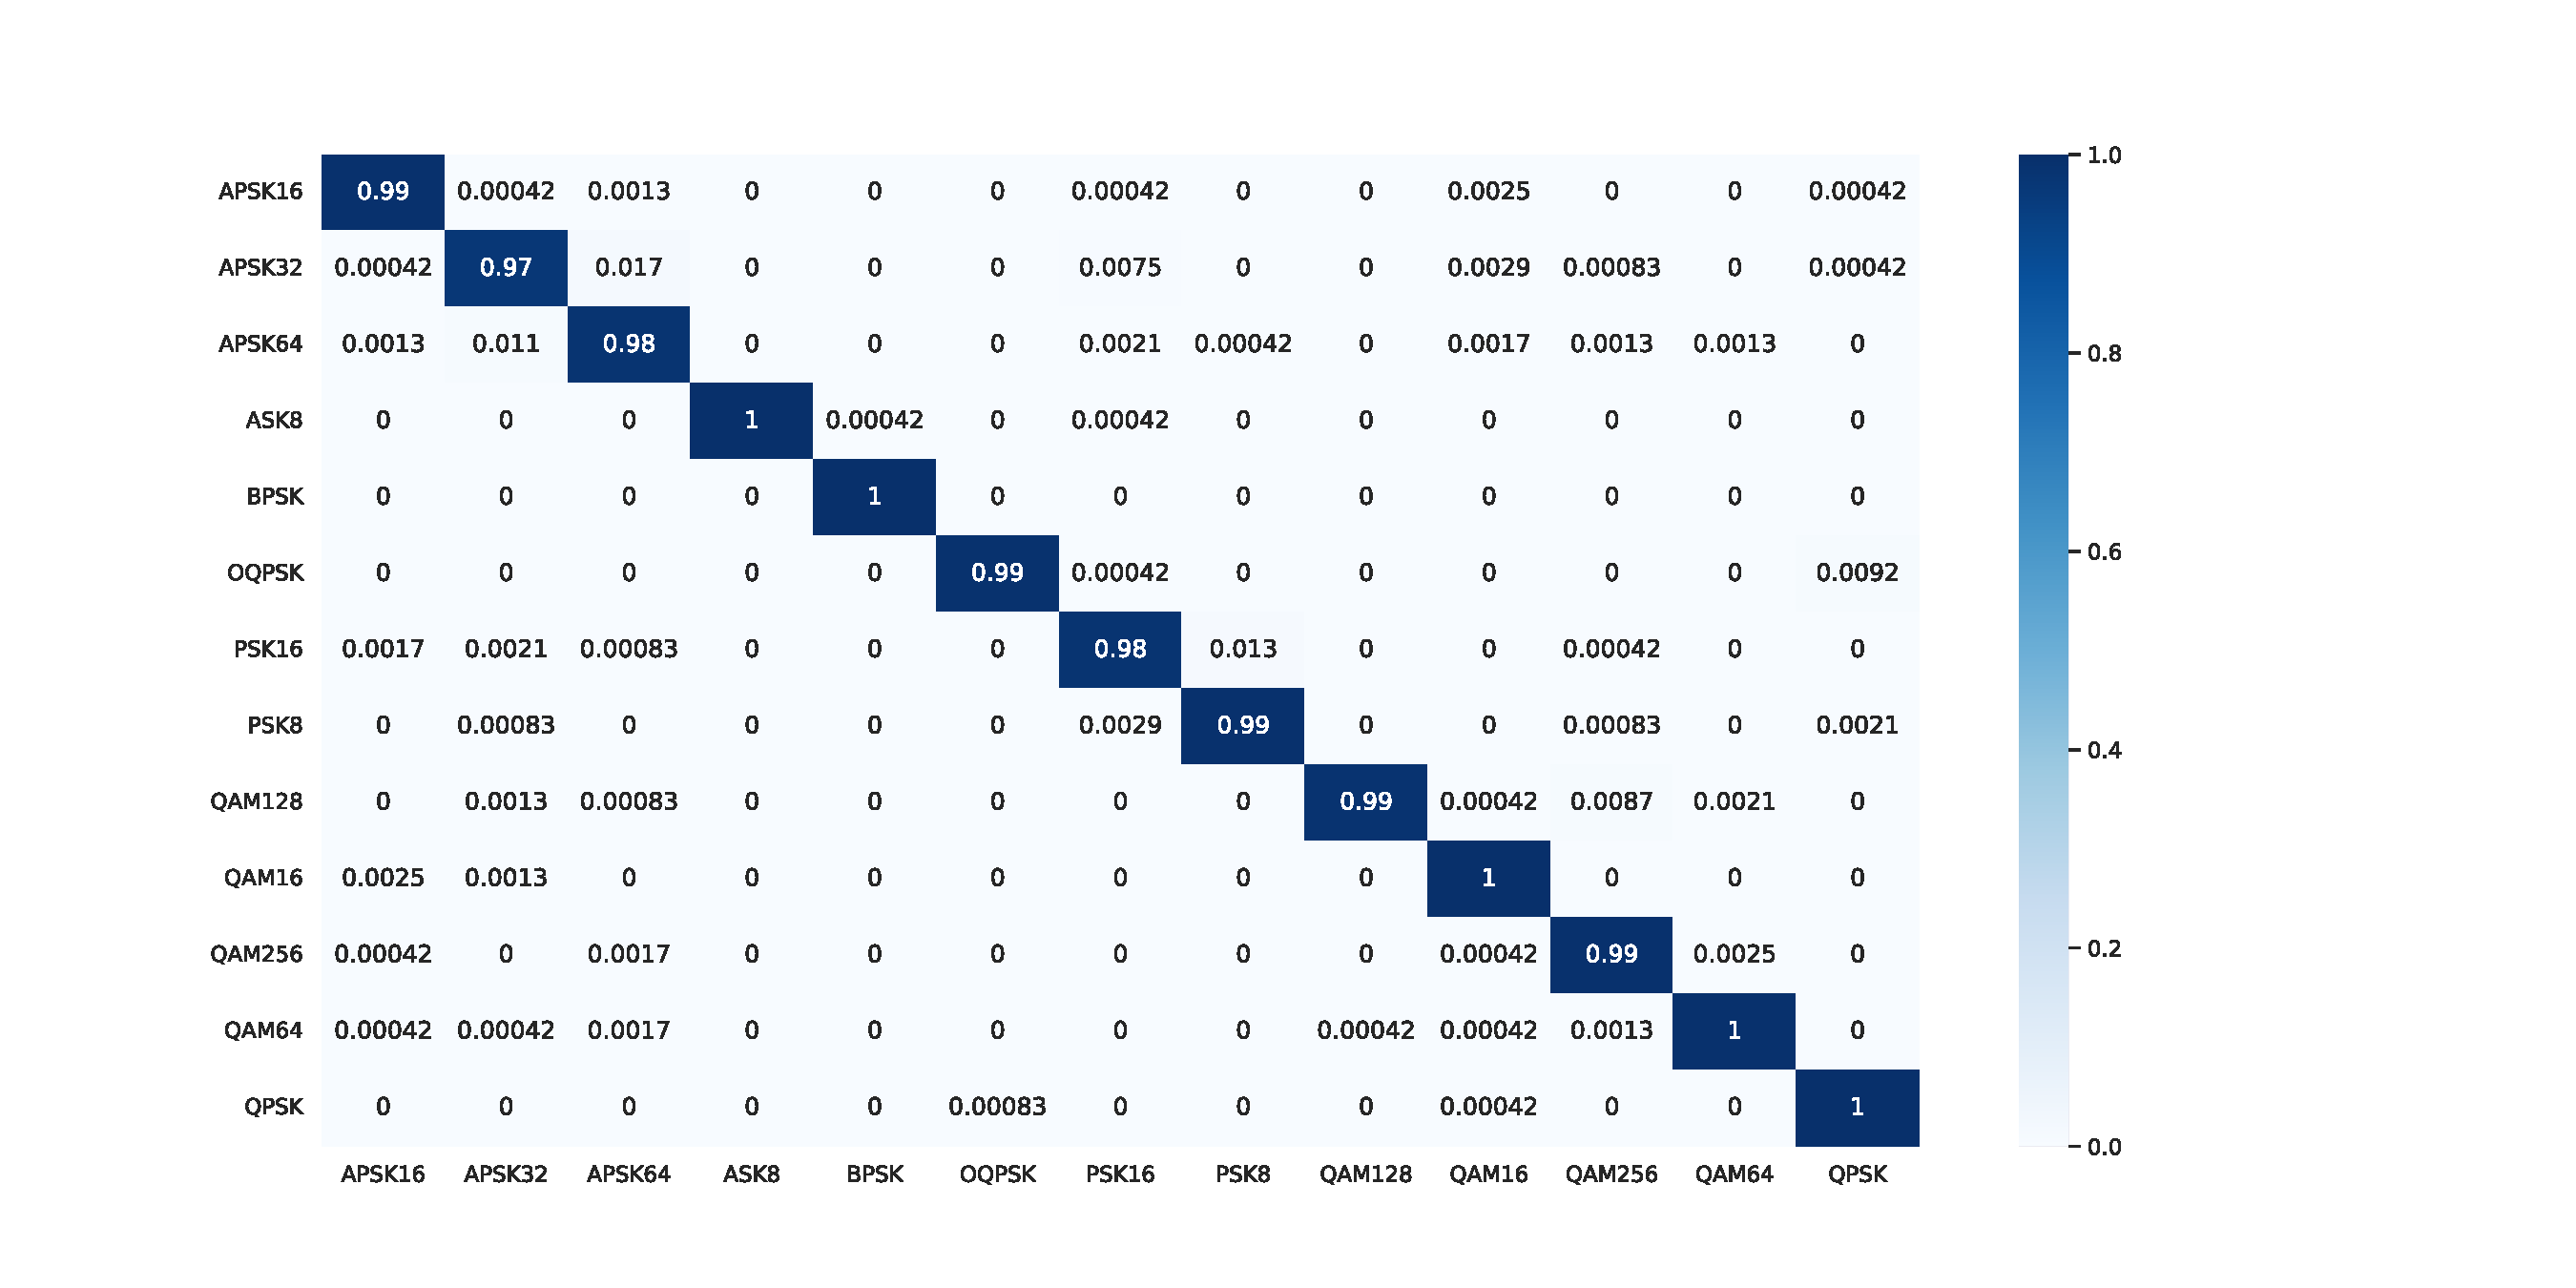
\includegraphics[width=\textwidth]{Image/confusion_matrix.pdf}
    \caption{单用户通信场景下的混淆矩阵(ResNet)}
    \label{fig:basic_result}
\end{figure}

\begin{table}[ht]
    \centering
    \caption{不同模型的性能比较}
    \label{tab:model_comparison}
    \begin{tabular}{lccc}
    \hline
    \textbf{模型}          & \textbf{参数量} & \textbf{训练至收敛的Epoch数} & \textbf{最终准确率} \\ \hline
    ResNet                 & 7.6M             & 68                           & 97.3\%              \\
    SE模块                 & 7.83M             & 57                           & 98.8\%              \\
    RSB模块                & 8.12M             & 54                           & 98.9\%              \\
    CBAM模块               & 7.96M           & 67                           & 98.5\%              \\
    多头自注意力机制模块 & 13.4M             & 99                          & 96.2\%              \\
    AD-AMR Net             & 1M            & 43                           & 99.8\%              \\ \hline
    \end{tabular}
    \label{tab:model_comparison_single_wideband}
\end{table}
    
从表\ref{tab:model_comparison_single_wideband}中提供的性能比较数据可以看出,不同模型在调制识别任务上的表现各有卓越。ResNet作为基线模型,已经展现了相当高的准确率(97.3\%),这验证了深度残差网络在特征提取方面的有效性。然而,通过引入注意力机制的模型在多数情况下能够实现更好的性能。

具体来说,SE模块和RSB模块以较小的参数增加(分别为7.83M和8.12M)实现了显著的性能提升,最终准确率分别达到了98.8\%和98.9\%。这表明通过重标定通道的重要性,可以更有效地利用模型的参数,从而提高准确率。CBAM模块虽然在参数量上仅略有增加(7.96M),但也展现出了良好的性能提升(最终准确率为98.5\%),证明了空间注意力和通道注意力的结合在提高模型敏感度方面的有效性。

多头自注意力机制模块的参数量显著增加至13.4M,但训练至收敛的Epoch数最高(99),且最终准确率相对较低(96.2\%)。这可能是因为该模块在处理一维信号时的参数并没有得到充分有效的利用,或者模型过于复杂导致过拟合。

显著地,我们提出的AD-AMR Net以极低的参数量(仅1M)和较快的训练速度(43 Epochs至收敛)达到了最高的准确率(99.8\%)。这一结果强调了AD-AMR Net在设计上的高效性和在调制识别任务上的出色性能,显示了在模型设计时对参数效率和网络结构优化的重要性。

总体而言,这些结果表明,通过引入针对性的注意力机制,可以在不显著增加参数量的情况下提升模型的性能。特别是,AD-AMR Net的优异表现证明了在保持模型轻量化的同时实现高准确度是可能的,这对于需要部署在资源受限环境中的调制识别系统尤为重要。
\section{宽带信号多用户调制识别}\label{sec:background}

% 在撰写宽带信号多用户调制识别这一章节时,您可以按照以下思路进行:

% 1. **多用户场景下的问题描述**:首先,详细介绍在多用户通信环境中识别调制信号的复杂性和技术挑战,特别是亚采样信号处理的复杂性。

% 2. **三种不同的解决方案**:
%    - **方案一(基线模型)**:根据子带的情况和各种调制的可能性,直接预测所有情况。简介该方案的实现及其作为基线的意义。
%    - **方案二(分步骤识别)**:首先识别子带的位置,然后在获取位置信息后进一步进行调制的识别。解释这种方法的步骤和预期效果。
%    - **方案三(多任务学习)**:总体对亚采样信号进行特征提取,然后使用不同的head分别进行子带位置的判别和调制模式的识别。阐述这种方案如何通过共用特征提取模块减少模型复杂度,同时增加两个子任务的关联性。

% 3. **实验设计和评估**:详细描述用于测试这三种方案的实验设计,包括数据集的选择、评估标准和实验流程。

% 4. **结果分析和比较**:展示每种方案的实验结果,并进行比较分析,以评估各方案的效果和适用性。

% 5. **讨论**:讨论所观察到的趋势和结果,探讨可能的改进方向和未来工作。

% 通过这样的结构,可以全面而深入地探讨多用户场景下宽带信号调制识别的各种策略和方法,展示实验研究的深度和广度。

\subsection{问题描述}\label{sec:background}

\begin{figure}
    \centering
    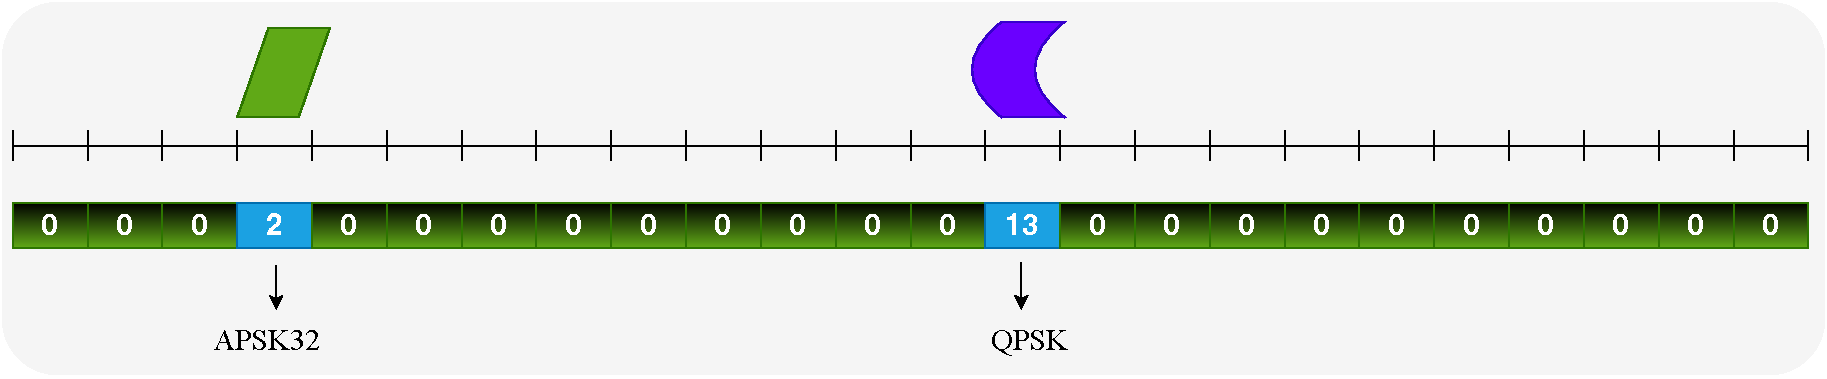
\includegraphics[width=\textwidth]{Image/mods.pdf}
    \caption{多用户通信场景下的调制识别问题描述}
    \label{fig:problem_description}

\end{figure}

在宽带多用户调制识别的问题描述中,我们面对一个复杂的通信环境,其中多个用户可能在相同或重叠的频率范围内同时传输信号。如图\ref{fig:problem_description}所示,这些信号可以被看作是分布在不同子带上的多个通道,每个通道可能采用不同的调制。例如,图展示了编号为2和13的两个子带正在被使用,而其他子带则处于空闲状态。在这种场景下,我们的目标是不仅识别出哪些子带正在被使用,而且还要准确地确定每个激活子带上的调制模式。在本研究的多用户宽带调制信号识别部分,所用数据集的采样形式保持与单用户场景一致,但在此基础上,数据集被构成为能够表示多个同时活跃信号的复合形式。具体来说,采样数据由多个不同延迟的模数转换器(ADC)收集,形成了一个$16 \times 1024$的矩阵。这个矩阵不仅包含了单一通信信号,还蕴含了多个信号的重叠,这些信号可能分布在不同的子带上,并可能采用与单用户场景中相同的13种调制类型之一。因此,数据集中的每个样本可能代表了一个或多个调制信号的组合,提高了识别的难度。此外,每个子带可能空闲或被不同调制模式的信号占据,这要求识别算法能够区分出哪些子带正在被使用以及它们各自使用了哪种调制模式。

这一任务的挑战在于,子带的识别和调制方式的分类需要在信号的亚奈奎斯特采样表示中进行,这要求我们的模型能够处理由不同延迟的ADC采集来的复杂信号。由于亚奈奎斯特采样可能导致采样数据的失真,这给准确识别调制信号带来了额外的难度。因此,我们必须设计出能够从亚奈奎斯特采样数据中提取关键特征,并执行准确分类的高效算法。

\subsection{实验方案}\label{sec:background}

\subsubsection{方案一:直接预测}\label{sec:background}

\begin{figure}
    \centering
    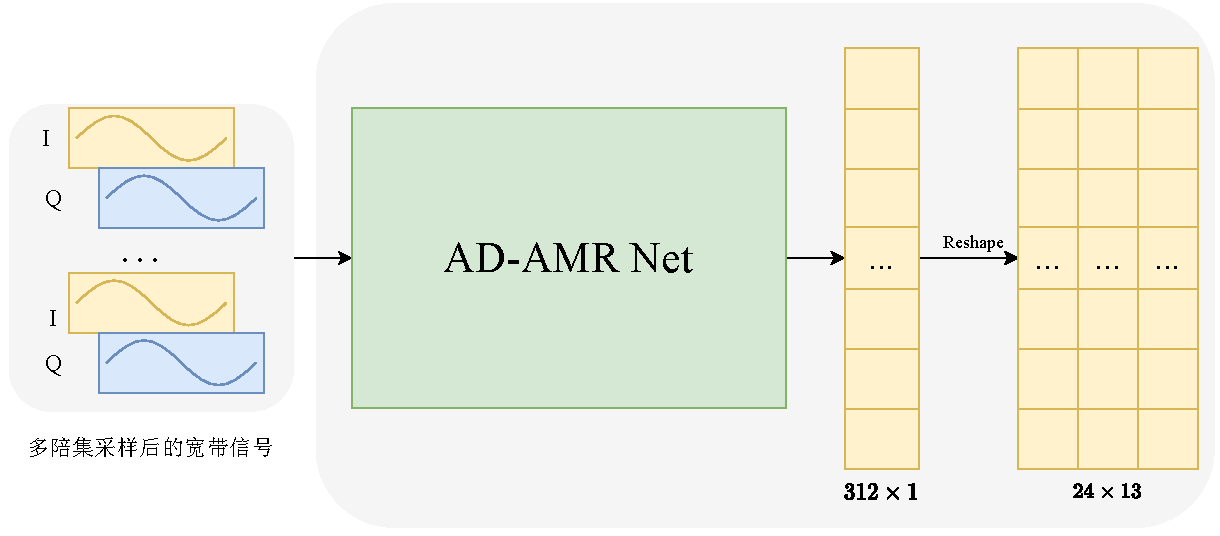
\includegraphics[width=\textwidth]{Image/plana.pdf}
    \caption{方案一:利用AD-AMR Net进行多用户场景下的宽带信号调制识别}
    \label{fig:plana}
\end{figure}

在多用户场景下的宽带信号调制识别的实验方案一中(如图\ref{fig:plana}所示),我们采用AD-AMR Net来处理分为24个子带的宽带信号,其中每个子带可能采取13种不同的调制模式或处于空闲状态。由此,模型面临的挑战是在这些子带中正确预测各种状态,总计达到\(24 \times 13\)种可能的情况。

实验的设计考虑到了信号的复杂性,尤其是在多用户环境下,信号的处理不仅需要准确识别调制模式,还需区分各个子带的特定状态。图\ref{fig:plana}展示了从接收的IQ信号开始,如何通过AD-AMR Net进行处理,并最终对每个子带的调制状态进行预测的简化流程。特别地,图中强调了信号预处理、网络处理以及重塑输出以适应大规模多分类任务的过程。

本次实验的主旨在于为整个研究建立一个性能基准线。在此方案中,网络性能的最优化并非首要目标,而是作为未来策略改进和比较的基础。此基线模型不仅提供了初始的性能指标,而且为后续采用更高级策略(例如分步骤识别或多任务学习方法)的效能评估提供了重要的比较基础。通过这种方法,我们可以清晰地定义后续方案需超越的性能门槛,并为评估AD-AMR Net在处理更复杂多用户场景时的潜力提供了一个参考点。


\subsubsection{方案二:分步骤识别}\label{sec:background}

\begin{figure}
    \centering
    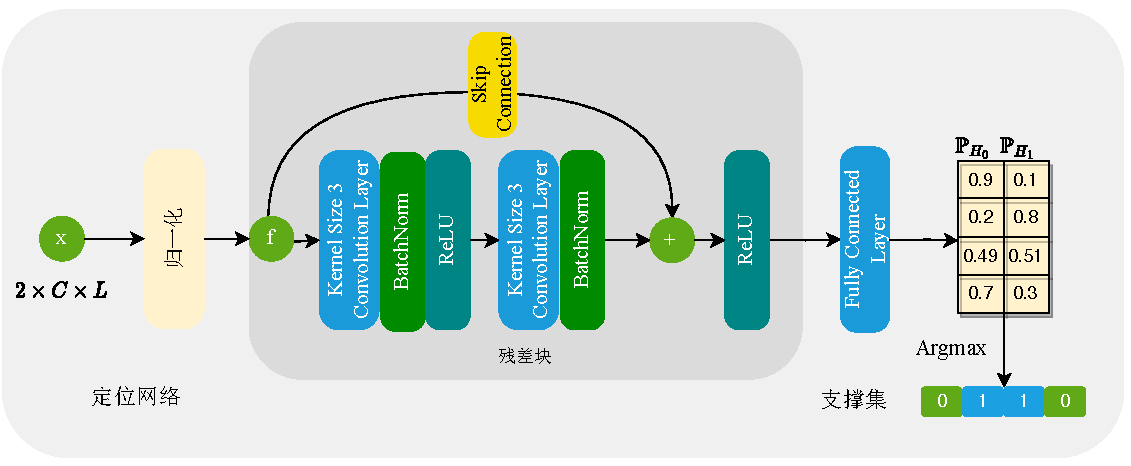
\includegraphics[width=\textwidth]{Image/localization.pdf}
    \caption{方案二中的定位网络架构,用于识别活跃子带}
    \label{fig:planb_localization}
\end{figure}

在这种策略中,问题被分解为两个主要步骤:子带活跃性检测(支撑集获取)和调制模式识别,每个步骤都由专门设计的网络处理。

如图\ref{fig:planb_localization}所示,定位网络首先接收信号作为输入,并通过一系列残差块和卷积层来处理信号。这个网络的设计重点在于利用残差连接和深层卷积网络的强大特征提取能力,以准确地定位哪些子带是活跃的。通过归一化和全连接层的处理,网络最终输出每个子带活跃与否的概率分数,这些分数随后被用于识别活跃的子带。

一旦活跃子带被成功识别,如图\ref{fig:planb_classification}所示的分类网络则负责进一步分析这些子带的调制模式。该网络采用了支撑集来处理已定位的活跃子带,并通过AD-AMR Net的高效特征提取和分类能力,实现对各种调制模式的精确识别。共享全连接层和归一化步骤确保了模型可以从子带特征中提取有用信息,并有效分类调制模式。

\begin{figure}
    \centering
    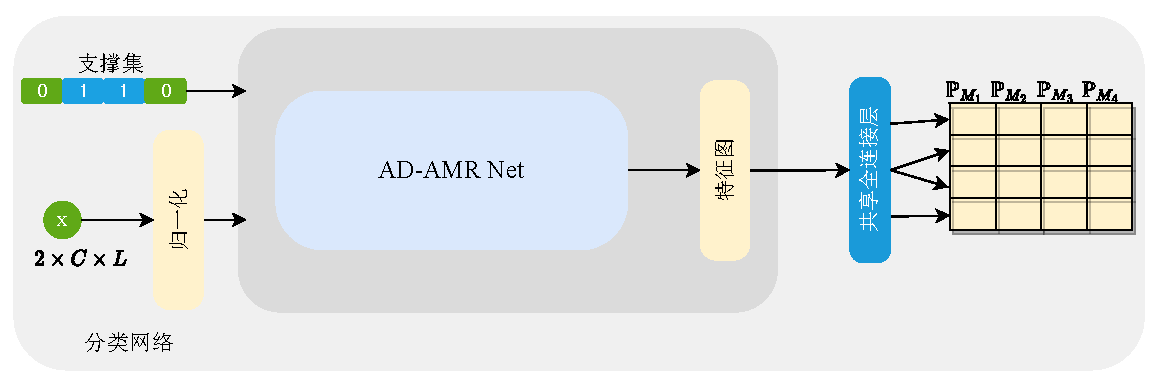
\includegraphics[width=\textwidth]{Image/classification_cn.pdf}
    \caption{方案二中的分类网络架构,用于识别活跃子带的调制模式}
    \label{fig:planb_classification}
\end{figure}

通过将调制识别问题分解为两个简化的任务,方案二不仅提高了识别的准确性,还增强了模型在多用户场景下的适应性和效率。定位网络和分类网络的结合,为解决复杂的宽带信号调制识别问题提供了一种有效且清晰的解决方案,展示了分步骤识别策略在提高性能和准确率方面的潜力。
\subsubsection{方案三:多任务学习}\label{sec:background}

\begin{figure}
    \centering
    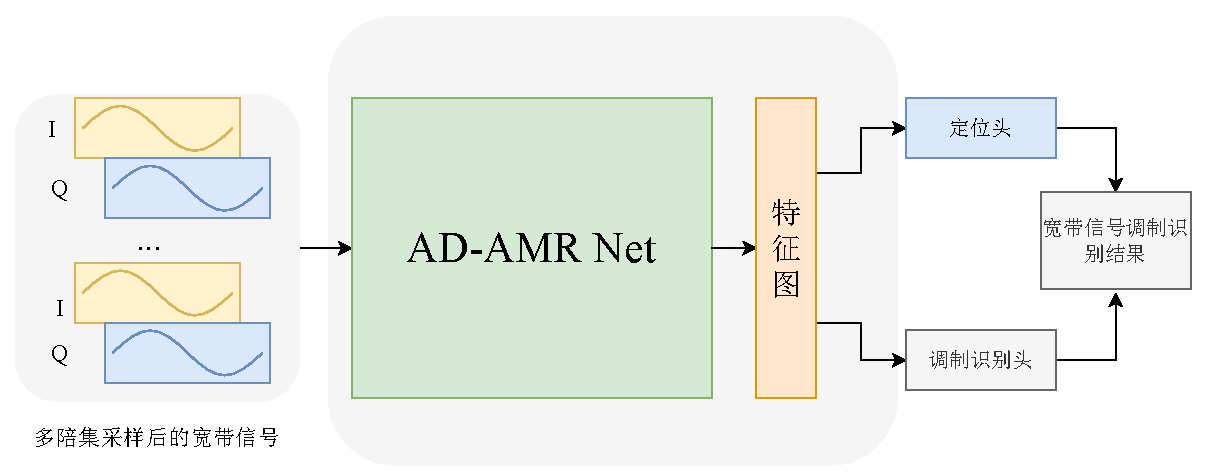
\includegraphics[width=\textwidth]{Image/planc.pdf}
    \caption{采用多任务学习方法进行宽带信号调制识别的方案三}
    \label{fig:planc}
\end{figure}
在方案三中,我们探讨了一种多任务学习方法,旨在通过单一的模型架构同时处理多用户宽带信号中子带检测和调制类型识别的双重任务。如图\ref{fig:planc}所示,这种方法的关键在于引入一个共享的特征提取模块,该模块能够捕获信号的全局特征,随后通过两个独立的任务特定头部(一个用于子带定位,另一个用于调制识别)来分别解决子带检测和调制类型识别的问题。

方案三的核心在于其高效的学习机制,通过共享特征提取模块捕获信号的全局特性,然后利用两个独立的任务特定头部同时进行子带检测和调制类型识别。这不仅降低了模型的复杂度,而且通过两个子任务的相互协作,增强了模型对复杂信号环境的适应能力。共享的特征提取模块使得模型能够在不同任务之间共享底层特征,从而提高了学习的效率和效果。

如图\ref{fig:planc}展示的,该方法首先对输入的IQ信号进行处理,通过AD-AMR Net提取信号的特征图,然后分别通过定位头和调制识别头进行子带活跃性检测和调制模式的识别。定位头负责判断哪些子带是活跃的,而调制识别头则针对检测到的活跃子带进行调制模式的精确识别。

通过这种设计,方案三实现了一种高效且灵活的方式来处理多用户场景下宽带信号的调制识别问题。通过多任务学习,模型能够在保持高性能的同时,更加高效地解决复杂的宽带信号处理任务,展现了多任务学习方法在提升识别准确性和模型效率方面的潜力。


\subsection{实验设计与评估}\label{sec:experiment_design_evaluation}

本研究的实验设计基于GBSense 2022 Advance数据集,旨在评估不同模型在多用户宽带信号调制识别任务上的性能。数据集提供了复杂的宽带信号样本,适合于测试模型在识别多种调制类型中的效能。

\paragraph{数据集} GBSense 2022 Advance数据集包括多种调制类型的信号样本,每个样本由24个子带组成,每个子带可能采用13种不同的调制模式或处于空闲状态,构成了一个高度复杂的多分类问题。

\paragraph{评价指标} 为全面评估模型性能,我们采用以下指标:
\begin{itemize}
    \item 子带活跃性检测准确率
    \item 调制类型识别准确率
    \item 总体识别准确率
    \item 模型参数量和计算效率
\end{itemize}

由于宽带信号中子带活跃性检测的困难性,我们引入了两种准确率指标,\textit{accuracy1}和\textit{accuracy2},以更细致地评估模型在此任务上的表现。

\begin{itemize}
    \item \textbf{\textit{accuracy1}(严格准确率)}:该指标要求模型的预测结果与实际状态完全一致才视为成功。例如,若实际子带活跃状态为$[0, 1, 1, 0]$,只有模型预测结果也完全为$[0, 1, 1, 0]$时,此预测才被认定为成功(计分为1);任何其他预测结果都视为失败(计分为0)。这种方式强调了完全准确的预测,不允许存在任何误差。严格准确率将被运用于最终准确率的评估中,以全面评估模型在子带活跃性检测任务中的性能。
    
    \item \textbf{\textit{accuracy2}(宽容准确率)}:考虑到任务的难度,\textit{accuracy2}提供了一种更为宽容的评估方法。若模型能完全准确预测子带的活跃状态(如预测$[0, 1, 1, 0]$且实际也为$[0, 1, 1, 0]$),则认为是完全成功(计分为2)。若预测结果部分接近实际情况(如实际为$[0, 1, 1, 0]$,预测为$[0, 1, 0, 0]$),则认为是部分成功(计分为1)。对于预测与实际情况差距较大的情况(如实际为$[0, 1, 1, 0]$,预测为$[1, 0, 1, 0]$),则视为失败(计分为0)。此方法允许一定程度的误差,同时根据预测的准确程度进行分级打分。宽容准确率将被用于神经网络的训练过程中,以确保训练时能够融合更多的信息。
\end{itemize}


考虑到宽带信号子带活跃性检测的稀疏性特点,即活跃子带相比非活跃子带在样本中出现的频率远低,我们采用了焦点损失(Focal Loss)作为训练神经网络的损失函数,以解决类别不平衡的问题。焦点损失的表达式为:

\begin{equation}
FL(p_t) = -\alpha_t (1 - p_t)^\gamma \log(p_t),
\end{equation}

其中,$p_t$是模型对于每个类别预测的概率,$\alpha_t$是针对每个类别的权重,$\gamma$是调整易分类样本贡献的聚焦参数。通过这种方式,焦点损失使模型更加专注于难以分类的少数类别,从而提高了在存在显著类别不平衡时的识别性能。

为了综合评估模型在子带活跃性检测任务上的表现,\textit{accuracy2}被采用作为评价指标。这种宽容准确率允许我们更加细致地衡量模型对于活跃子带预测的准确性,同时考虑到完全正确和部分正确的预测。通过结合使用焦点损失和\textit{accuracy2}评价指标,我们旨在促进神经网络在处理类别不平衡且具有挑战性的宽带信号子带活跃性检测任务中的训练效率和性能。


\paragraph{实验设置} 实验在Ubuntu操作系统上基于PyTorch框架进行,利用NVIDIA RTX 3090 GPU进行加速。我们遵循标准的数据集划分比例(训练集60\%,验证集20\%,测试集20\%),并设置所有模型训练至少100个epochs,采用早停机制防止过拟合,同时也采用了平台期衰减学习率来动态调整学习率。为了优化模型性能,使用随机梯度下降(SGD)优化器和交叉熵损失函数进行训练。

\paragraph{实验方案简述} 本研究设计了三种实验方案:基线模型(方案一)、分步骤识别(方案二)、和多任务学习(方案三)。这些方案被设计来探索不同策略对提高多用户宽带信号调制识别效率和准确率的影响。通过比较这些不同方案的性能,我们期望得出哪些策略在实际应用中最为有效,从而为后续的研究和实际部署提供指导。

通过这套综合的实验设计和评估标准,我们旨在深入理解不同策略在解决复杂的调制识别任务中的潜力和限制,为未来宽带信号处理的研究提供实验基础和理论支撑。



\subsection{结果分析}\label{sec:background}

\begin{table}[ht]
    \centering
    \caption{不同模型的性能比较}
    \label{tab:model_performance}
    \resizebox{\textwidth}{!}{
    \begin{tabular}{lcccc}
    \hline
    \textbf{方案} & \textbf{模型参数量} & \textbf{收敛Epoch数} & \textbf{子带活跃状态Accuracy1} & \textbf{调制识别Accuracy1} \\ \hline
    方案一 & 8.9M & 74 & 99.9\% & 23.8\% \\
    方案二 & 2.7M & 31 + 56 & 99.9\% & 87.1\% \\
    方案三 & 1.6M & 64 & 99.9\% & 94.3\% \\
    \hline
    \end{tabular}
    }
\end{table}

根据表\ref{tab:model_performance}中的结果,我们可以进行以下分析:

方案一,作为基线模型,拥有8.9M的模型参数量和需要74个Epochs才能收敛。尽管在子带活跃状态检测上达到了极高的准确率(99.9\%),表明模型能够非常准确地判断子带是否活跃,但在调制识别任务上的表现相对较弱,仅有23.8\%的准确率。这表明单一策略在处理复杂的调制识别任务时可能面临挑战,尤其是在没有专门针对调制识别优化的情况下。

方案二采用了分步骤的识别方法,显著减少了模型参数量至2.7M,并以两阶段的训练过程(分别为31个和56个Epochs)达到收敛。这种方法同样在子带活跃状态检测上取得了99.9\%的高准确率,同时在调制识别任务上的表现大幅提升至87.1\%。这一改进证明了通过将问题分解为两个相对简单的任务,模型能够更专注于各自的挑战,从而提高特定任务的识别准确率。

方案三通过实施多任务学习策略,进一步降低了模型的参数量至1.6M,且在64个Epochs内达到收敛。该方案在子带活跃状态检测上同样实现了99.9\%的准确率,并且在调制识别任务上达到了94.3\%的高准确率,表现最佳。这一结果突显了多任务学习在提高模型对复杂信号处理能力的同时,还能维持高效的模型规模和较快的训练速度。

综上所述,虽然所有方案在子带活跃状态检测上均表现出色,但在调制识别准确率上,采用分步骤识别(方案二)和多任务学习(方案三)的策略明显优于单一策略(方案一)。尤其是方案三,不仅在调制识别任务上达到了最高准确率,而且具有最低的模型参数量和相对较快的收敛速度,展现了在处理多用户宽带信号调制识别问题时的显著优势。这些发现为未来在类似任务上的模型选择和策略优化提供了重要的参考和指导。

\section{宽带信号调制解调}\label{sec:mod_demod}

随着多任务学习策略在宽带信号调制识别任务中取得显著进展,我们进一步探索了该策略在调制信号解调方面的应用。本节将详细介绍该策略在处理单用户和多用户宽带信号调制解调任务中的应用和潜力。

\subsection{单用户宽带信号调制解调}


\begin{figure}
    \centering
    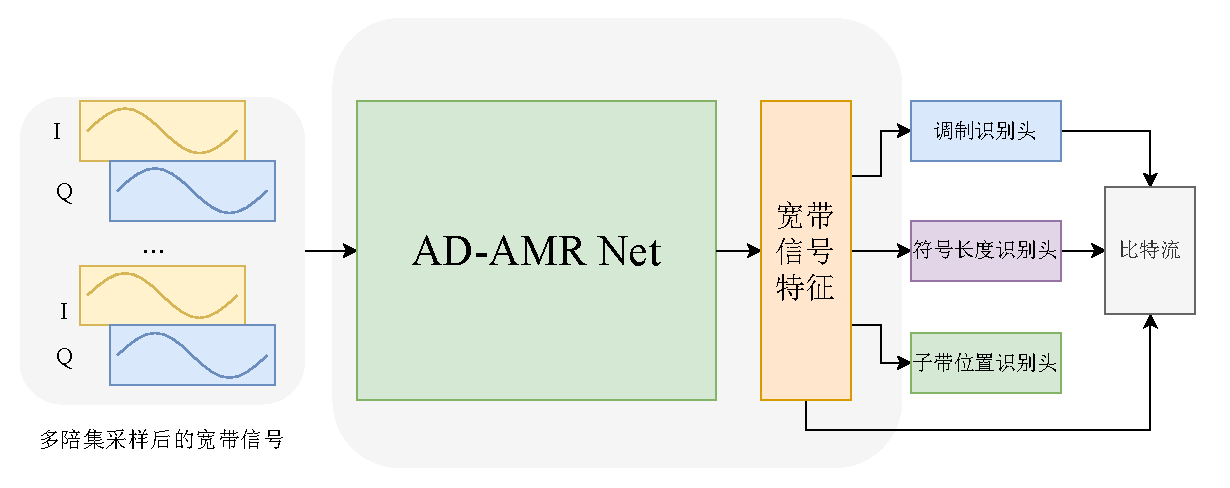
\includegraphics[width=\textwidth]{Image/adamr-wideband_demodulate.pdf}
    \caption{单用户场景下的调制解调流程图}\label{fig:demode_single}
\end{figure}

对于单用户场景,本研究采用GBSense 2023 Basic数据集进行实验。该数据集提供了丰富的单用户宽带信号样本,涵盖了多种调制模式,为深入研究调制解调技术提供了理想的测试平台。通过利用多任务学习策略,这部分实验不仅旨在准确识别信号的调制类型,还致力于从调制信号中准确恢复出原始信息,以评估和验证该策略在解调过程中的有效性和效率。该实验的主要思路如\ref{fig:demode_single}所示,具体来说,通过多任务的神经网络先使用一个共享的网络来提取信号特征,然后用不同的头(卷积层)来提取信号的其他信息(调制模式、符号长度等)。结合这些信息能够得到比特流的长度,最后结合主干网络所学习到的特征以及比特流的长度信息,最终可以获取所解调信号的比特流。

\subsection{多用户宽带信号调制解调}
\begin{figure}
    \centering
    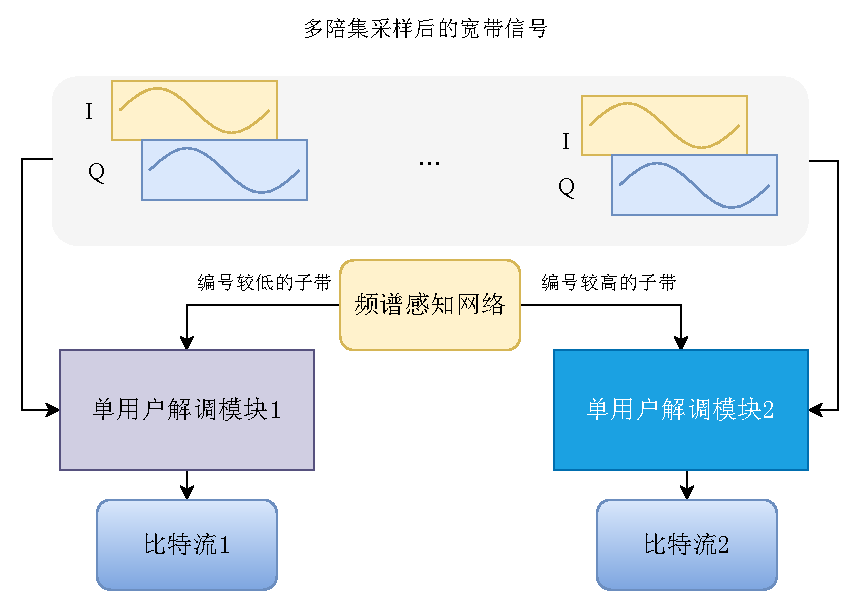
\includegraphics[width=0.8\textwidth]{Image/adamr-wideband_demodulate_mul.pdf}
    \caption{多用户场景下的调制解调流程图}\label{fig:demode_multiple}
\end{figure}

针对多用户场景,我们使用GBSense 2023 Advance数据集作为研究基础。相较于单用户场景,多用户宽带信号的调制解调任务在复杂度上有所增加,因为需要同时处理来自多个用户的信号,并准确地区分和解调各自的调制信号。多任务学习策略在此场景下的应用,旨在通过共享的特征提取模块捕获信号的全局特性,并利用任务特定的子模型分别进行子带检测和调制类型识别,从而实现高效准确的调制解调性能。如图\ref{fig:demode_multiple}所示,该策略的核心在于采取了“分而治之”的策略,先通过一个频谱感知网络获取信号的全局特征和支撑集信息,然后将信号分别送入两个独立的解调网络进行解调,在这里的解调网络和之前的单用户场景下的网络结构整体上是一直的,在训练时,各个子解调模块只专注于属于自己子带编号上的信号解调,这样能够有效提高解调的准确性。

\subsection{实验设计与结果}

\subsubsection{单用户宽带信号调制解调实验}

由于是多任务模型,该实验的评价指标将结合各个子任务的性能来探究。
\begin{itemize}
    \item \textbf{误码率 (Bit Error Rate, BER)}:评估解调后的比特流中错误比特的比率。
    \item \textbf{信号长度识别准确率 (Length Accuracy)}:评估模型预测信号长度的准确性。
    \item \textbf{调制类型识别准确率 (Modulation Accuracy)}:评估模型识别调制模式的准确性。
    \item \textbf{符号长度识别准确率 (Symbol Length Accuracy)}:评估在符号级别上模型预测信号长度的准确性。
\end{itemize}

经过训练和测试,模型在单用户宽带信号调制解调任务上取得如表\ref{tab:performance_metrics}所示。
\begin{table}[ht]
    \centering
    \caption{性能指标概览}
    \begin{tabular}{l|c}
        \hline
        \textbf{性能指标} & \textbf{数值} \\
        \hline
        比特错误率 & 0.08423166826246754 \\
        信号长度识别准确率 & 0.9613283125 \\
        调制类型识别准确率 & 0.9762173502441833 \\
        符号长度识别准确率 & 0.98077253547484202 \\
        \hline
    \end{tabular}
    \label{tab:performance_metrics}
\end{table}

    

实验结果表明,AD-AMR Net在单用户宽带信号的调制解调任务上表现优秀,特别是在调制类型和符号级长度的识别上。这一结果为单用户宽带信号解调提供了一种有效的解决方案,同时验证了多任务学习策略在解决此类复杂信号处理问题中的潜力和实用性。

\subsubsection{多用户宽带信号调制解调实验}

多用户场景的评估指标与单用户场景类似,但在多用户场景下,模型需要处理来自多个用户的信号,在GBSense 2023 Advance数据集中,每个用户的信号都有不同的子带编号,因此模型需要能够准确识别子带的编号并解调对应的信号。实验结果如表\ref{tab:multi_user_module_performance}所示。

\begin{table}[ht]
    \centering
    \caption{多用户模块性能指标}
    \begin{tabular}{l|c|c}
        \hline
        \textbf{性能指标} & \textbf{低子带} & \textbf{高子带} \\
        \hline
        比特错误率 & 0.12516188621520996 & 0.17647825956344604 \\
        信号长度识别准确率 & 0.9600694179534912 & 0.9504687237739562 \\
        调制类型识别准确率 & 0.9769096970558167 & 0.9769096970558168 \\
        符号长度识别准确率 & 0.9790364503860474 & 0.8517617118358612 \\
        \hline
    \end{tabular}
    \label{tab:multi_user_module_performance}
\end{table}

在我们针对多用户模块性能的评估中,考虑到了两个子带:高子带和低子带。性能指标包括比特错误率(BER)、信号长度识别准确率、调制类型识别准确率以及符号长度识别准确率。根据结果,我们注意到,虽然调制类型识别准确率和信号长度识别准确率在两个子带上表现出了较高的准确性,但比特错误率(BER)的表现并不尽如人意。

BER是衡量系统性能的一个核心指标,它直接反映了信号传输过程中的错误率。在多用户场景下,我们处理的是混叠的宽带信号,这些信号的复杂性显著增加了识别的难度。此外,压缩采样率等因素也对BER产生了不利影响。尽管我们采取了多种措施来优化系统性能,但在面对多用户环境下的宽带信号处理时,这些挑战是预期之中的。我们认识到,高BER反映了在当前技术条件和系统架构下,信号处理的固有限制。

综上所述,尽管我们在调制类型识别准确率和信号长度识别准确率等方面取得了良好的成绩,但在比特错误率上的表现突显了在多用户场景下处理混叠宽带信号的复杂性。这些结果激励我们进一步探索新的技术和方法,以提高系统在处理高度复杂信号时的性能,同时也提醒我们在未来工作中需要更加关注BER的改进。


\section{本章总结}\label{sec:background}
在本章中,我们深入探讨了宽带信号多用户调制识别的问题。面对复杂的多用户通信环境,我们提出并测试了三种不同的策略来解决宽带信号的调制识别问题。

首先,我们实现了一个基线模型,该模型直接预测所有可能的子带位置和调制类型组合。这种方法为我们提供了一个初步的性能基准,虽然简单但在某些情况下能够有效工作。随后,我们探索了一种分步骤的方法,先识别子带位置,再进行调制识别。这种策略使我们能够更精细地处理信号,提高了识别的准确性。

最后,我们采用了一种多任务学习策略,该策略在总体上对亚采样信号进行特征提取,然后通过不同的头实现子带位置的判别和调制模式的识别。这种方法通过共用特征提取模块减少了模型的复杂度,并增加了两个子任务的关联性,从而在保持高效率的同时提高了识别的准确度。

受到宽带调制识别中多任务方法的启发,我们进一步拟出并实现了对亚采样宽带信号直接解调的框架,在单用户场景下取得了一定的成果。这一新策略不仅补充了之前方法的局限性,还拓宽了我们对宽带信号处理能力的认识。

通过对这些方法的实验评估,我们不仅验证了它们在多用户宽带信号调制识别任务中的有效性,还展示了各种策略的优势和局限性。这些实验结果为未来在宽带信号处理和调制识别领域的研究提供了有价值的见解,特别是在设计适应复杂通信环境的算法时。我们相信,本章的研究工作将对未来的技术发展和应用实践产生积极影响,为处理更为复杂的通信系统中的挑战提供了可行的解决方案和方法。
